%%%%%%%%%%% Aquí va la solución al problema 1.
\newpage
\textbf{\textcolor{MidnightBlue}{1.}} Considera la siguiente variante del algoritmo
de consenso con terminación temprana.
Contesta lo siguiente:
\begin{enumerate}[a)]
    \item Demuestra que el algoritmo 1 soluciona el problema del consenso,
    tolerando $f < n$ fallas de tipo paro, donde $n$ es el número de procesos en el sistema.

    Por demostrar:
    \begin{itemize}
        \item Terminación

        El algoritmo no tiene una clara condición de salida. La linea 6 se
        ejecutara indefinidamente, a menos que exista una en la linea 9 cuando
        se ejecuta \textit{decide max(vista)}.

        \item Validez

        El valor de \textit{prop = vista} fue propuesto por algún proceso en cada ronda.

        \item Acuerdo.
        No queda claro si el algoritmo termina, sin embargo:
        Veamos una ejecución cuando $f=0$:
        Al inicio de la ejecución $r=0$, la \textit{flag = false},
        envía $<prop,false>$, luego $r=1$,
        $vista = prop, prop_1$, luego
        $rec[1]= 1+1$ y no se modifica \textit{flag}
        hasta que $rec[1-1]==rec[1]$,
        en esta ronda no se modifica \textit{flag}


        Cuando $r=2$,
        $send(<prop_2,false>)$ a todos
        \textit{vista = \{$prop,prop_1,prop_2$\}}
        $rec[2]=1+1$

        $rec[2-1]==rec[2] \rightarrow rec[1]==rec[2]$, en esta ronda se modifica $flag=true$


        Cuando $r=3$,
        $send(<prop_2,true>)$ a todos
        \textit{decide max(vista)}
        \textit{vista = \{$prop,prop_1,prop_2,prop_3$\}}
        \textit{ dec = true}
        $rec[3]=1+3$
        $rec[3-1]==rec[3] \rightarrow rec[2]==rec[3]$, en esta ronda no se modifica $flag=true$


        Cuando $r=4$,
        $send(<prop_3,true>)$ a todos
        \textit{decide max(vista)}
        \textit{vista = \{$prop,prop_1,prop_2,prop_3,prop_4$\}}
        \textit{dec = true}
        $rec[4]=1+3$

        $rec[4-1]==rec[4] \rightarrow rec[3]==rec[4]$, en esta ronda no se modifica $flag=true$

        Si algún proceso tuviera una falla de tipo paro, el valor de vista sería
        diferente y si al menos una flag de la ronda anterior es verdadera entonces
        llega a un acuerdo con los valores de vista. Por lo tanto en cada dos
        rondas a partir de la tercera, todos los proceso (vivos) acuerdan el mismo valor.
    \end{itemize}


    \item ¿Es cierto que los procesos correcto terminan en a lo más
    $max(t +2, f +1)$ rondas en el algoritmo 1? Argumenta tu respuesta.
    Recuerda que $t \leq f$ es el número de fallas que realmente ocurren en una
    ejecución dada.\\
    Si $t$ es el número de fallas que realmente ocurren en una ejecución y $f$ es el número de fallas de tipo paro.
    Notemos que el algoritmo toma dos rondas para poder llegar a consenso: en la primer ronda recibe los mensajes y los almacena en la variable $vista$ por la linea 10. Aplicar $or$ a las flags que al momento son $false$, y luego al verificar $rec[r-1]==rec[r]$ y actualice $flag=true$. Para que en la segunda ronda decida el $max$ a partir de $vista$, la cual es la union de las vistas propuestas por los procesos en la ronda uno.

    De manera similar al algoritmo del consenso visto en clase se tardara $t+1$ rondas en llegar a un consenso pero notemos que si encontramos un error más de los esperados son necesarias dos rondas más para llegar a un consenso.

    \item Haz un análisis del número máximo de mensajes que se envían en una
    ejecución del algoritmo 1. Tu cota debe estar en función de $n$ y $f$.

    El número de mensajes máximo se puede expresar como la suma de todos los mensajes recibidos por cada proceso en cada ronda, lo cual es almacenado en cada ronda en la variable \textit{rec[r]} en la linea 14
    \[\sum_{i=0}^r rec[i] = 1+rec[0]+1+rec[1]\]
\end{enumerate}

\newpage
\begin{figure}
    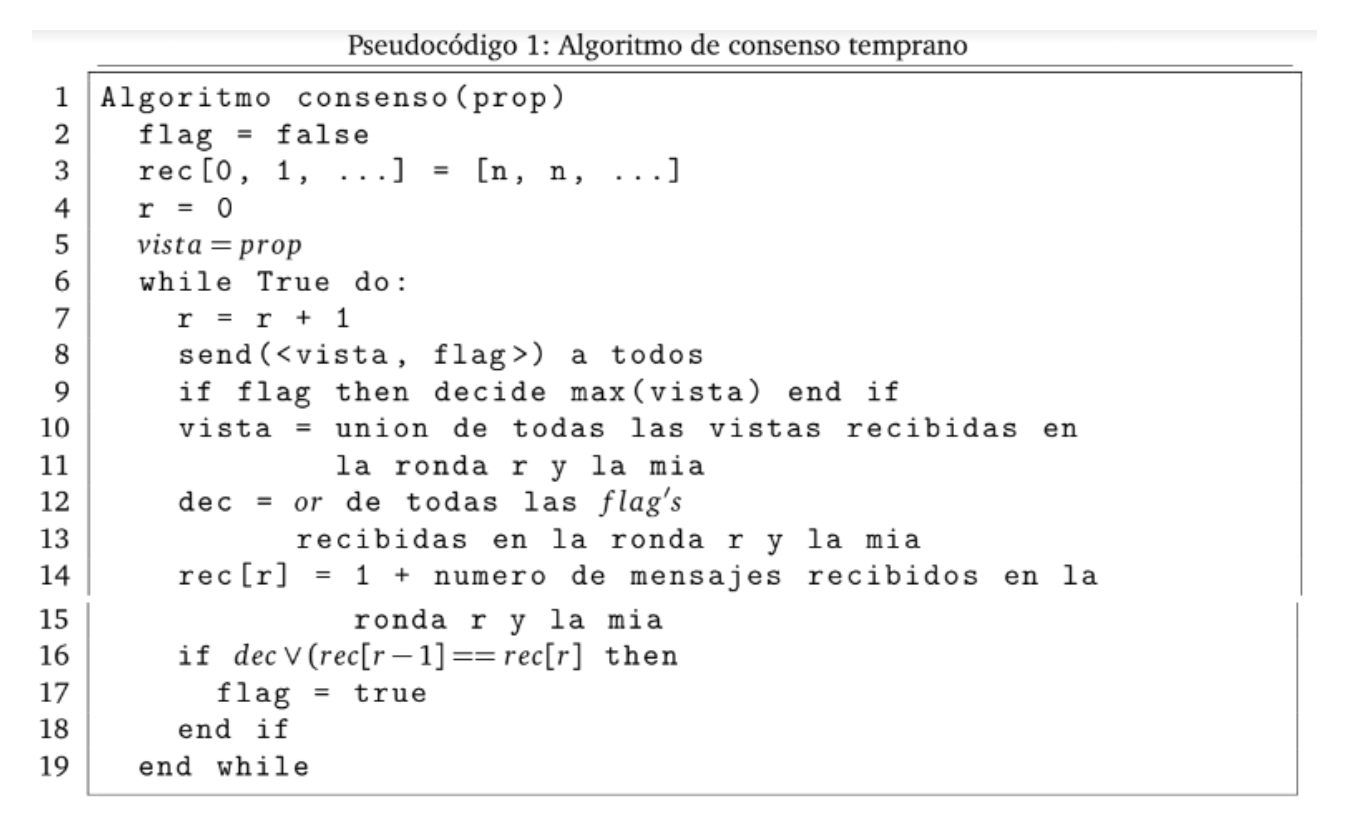
\includegraphics[width=\textwidth]{consensoTemprano.png}
\end{figure}
